\chapter{Analysis}
\label{analysis}
This chapter contains discussion of different approaches for meeting the desired requirements. If also provides the arguments for the selection of some specific libraries later used in the thesis. It starts with a section summarizing the limitations of the similar monitoring solutions and is followed by several sections where each of these sections is dedicated for a single requirement. The requirement sections discuss in more detail what solution is the best for meeting the desired requirement. This chapter ends by a summary of the wanted and unwanted features in more detail compared to the few basic requirements.

\section{Limitations of Similar Solutions}
This thesis tries to overcome some of the limitations of the relevant monitoring tools and give the users the alternative solution. One goal of this tool is to be an open-source solution which is in contrast to the proprietorial \hyperref[dapper]{Google Dapper}. Google Dapper is also targeted to only specific type of applications sharing the same code structure and libraries used at Google and therefore there is a certain lack of the universality. 

\hyperref[zipkin]{OpenZipkin} is stable open-source tracing system. Zipkin creates several pre-instrumented libraries which may be used at the monitored application to communicate with the Zipkin backed. These libraries try to minimize the amount of code changes in application sources, however the user is still required to change the application source code to add custom annotations or change the default tracing mechanism. The similar holds for very similar tool developed by Cloudera, \hyperref[htrace]{HTrace}. These tools also perform the instrumentation in the same JVM (Java Virtual Machine) where the application is running which can have performance impact on the application itself.

The tool proposed by this thesis tries to address these problems and find solutions how applications can be instrumented without the need of changing the source code and have the minimal performance impact on the running application.
\section{Requirement - Small Footprint and High Performance}
The mentioned cluster monitoring tools can affect the application performance and memory consumption since they perform instrumentation in the same virtual machine as the monitored application. One of the thesis requirements is to have  a minimal footprint on the monitored application.

Since the instrumentation is a core functionality of the system it directly affects the performance of the application. Different instrumentation methods are described in the following few paragraphs to give the reader insights into how each method can affect the application's performance. Two standard ways of instrumentation exist - using the native or Java agent and the advantages and disadvantages of these two approaches are discussed here together with the arguments for the final solution which is actually a compromise of the both techniques.
\subsection{Java Agent}
\label{java_agent}
Java agents are used for instrumenting the applications on the Java-language level where the user does not need to worry about the JVM internals. Usually, the programmer extends and creates custom class file transformers and the agent internals take care of applying the code when required. 

The advantage of this approach is obvious - the ability to write the instrumentation in the high-level language without the knowledge of the underlying byte code. The distributions of Java Agents is also platform independent since they are packaged inside JAR (Java ARchive) files as the rest of Java classes. 

The disadvantages of this approach are usually the performance and the flexibility of the agent. Objects created by Java agents are affected by garbage collection of the monitored application and thus can have negative impact on the application itself. Also the objects created from the agent are put on the application's heap and therefore consume the applications' memory. For the reasons above, it can happen that the observed information via Java Agent can be influenced by the monitoring process itself. Java agents also can not be used to respond to internal JVM events and it is important to note that Java system classes can not be instrumented when using this method.
\subsection{Native Agent}
Native Agent are used for monitoring and instrumenting the applications in the low-level programming language (C, C++) using \hyperref[JVMTI]{JVMTI} and \hyperref[JNI]{JNI}. Native agents are written as native libraries for specific platforms and therefore the packaging is not platform independent. 

The disadvantage of this method can be that the agent has to be written in non-Java language, but on the other hand this approach gives the developer the full flexibility in the instrumentation and monitoring of the JVM state. For example, even the System classes can be instrumented using this approach and callbacks may be created to respond to several JVM internal events such as start or end of the garbage collection process, creation of new instance of specific class or switching threads. The native agent is running as part of the Java process and therefore any resource-demanding computation can have negative performance impact on the application's performance as well as in the \hyperref[java_agent]{Java Agent} method. However objects created in the native agent are not subject to garbage collection and are not created on the heap except when created using \hyperref[JNI]{JNI} in the target Java application.

The significant technical disadvantage of this approach is that it does not provide any helper methods to help with the code instrumentation and generally, the is a lack of stable instrumentation libraries written in C++ or C which could be used inside the agent. The developer of the native agent has therefore write all the required methods for extracting the relevant parts of the byte code and the instrumentation itself.
\subsection{Chosen Method}
\label{subsec:inst_jvm}
The desired solution should be able to instrument the code without affecting the performance and memory of the monitored application whilst still having access to internal JVM state and allowing the developer to use high-level programming language to write the instrumentation code. For these reasons the compromise between the proposed solution has been chosen together with introduction of special process used specifically for the instrumentation. The solution can be seen on the figure \ref{fig:inst_server_basic}.
\begin{figure}
	\centering
	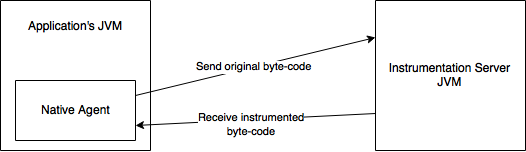
\includegraphics[scale=0.7]{inst_server.png}
	\caption{Sketch of the chosen approach.}
	\label{fig:inst_server_basic}
\end{figure}

In more detail, the native agent is used to to communicate with the application being monitored. When a class needs to be instrumented, the native agent sends the class's byte code to special instrumentation Server JVM. This machine handles the instrumentation and sends the instrumented byte code back to the native agent. Therefore the native agent is only used to collect important internal JVM information, send classes for instrumentation and receives the instrumented classes back. The instrumentation does not happen in the same JVM as the monitored application which allows the tool to have minimal performance impact on the application. Also, since the instrumentation is not done in the native agent  but in the instrumentation server based on Java, this machine can use any of the available byte code manipulation tools which operates on Java-language level and thus there is no need to implement the byte-code manipulation library completely from scratch in the native agent. Another advantage of this solution is that even the application's Java system classes may be instrumented in Java language on the instrumentation server.

Byte Buddy library was selected for the byte code manipulation within the instrumentation server  as it allows to write the instrumentation in Java without the deep knowledge about the Java byte code which is necessary when using \hyperref[asm]{ASM} library. Also, the library is supposed to have really good performance results based on the official benchmarks available on the library's page. Compared to \hyperref[javassist]{Javassist}, the code is not written inside Java Strings, which means that the instrumentation code can be validated in today's IDE during compilation time and bugs in the instrumentation code can be found easier. The API of the library is well-documented, compared to \hyperref[cglib]{CGLib}, and the library is under active development. Byte Buddy is also highly configurable library which was also the significant reason for choosing it as the tool for instrumenting classes inside different JVM then where they are actually used. Achieving the instrumentation in the secondary JVM  turned out to be challenging part of the thesis and the technical aspects of the solutions are described later in the thesis.

The disadvantage of the chosen approach is that the native agent has to send the byte code to the instrumentation server and wait for the instrumented byte code. However several optimizations have been implemented to minimize this delay as much as possible. More information about these optimizations can be found in the \hyperref[sec:inst_server]{Instrumentation} section of \hyperref[chap:design]{Design} chapter.
			
\subsection{Alternative solutions}
Two alternative instrumentation solutions were analyzed but rejected at the end. The first alternative solution was to perform the instrumentation right in the agent even for the price of affecting the application's performance by instrumenting in the same JVM. However this solution required to write the instrumentation from scratch in C++ or C language since there are no stable libraries for this purpose. Even though this would be possible, it would take significant amount of time and also, it was not aimed of the thesis to create such a library. The performance impact on the application's was also important reason for rejecting this method.

The other alternative solution was based on the idea of running multiple Java Virtual Machines inside one native process. In particular, running the application and the instrumentation server inside the same process. This would have the same  negative performance impacts as the solution above, however it would allow the developer to perform the instrumentation in Java programming language compared to C++ or C. Also all the communication between the machines would be only inside one single process compared to the chosen solution where the communication needs to be handled over the network or between different processes. However, as of JDK/JRE 1.2, creation of multiple virtual machines in a single process is not supported \cite{MoreJVMOnceProccess}.
							
\subsection{Chosen Communication Layer}
The selection of the tool used for the communication between the native agent and the instrumentation server was also important decision and \hyperref[nanomsg]{NanoMsg} has been chosen. It hides the platform specific aspects of sockets comparing to \hyperref[raw_sockets]{Raw Sockets} approach. It has also several performance benefits and general improvements over the well-known \hyperref[zeromq]{ZeroMq} library such as the better threading and more sophisticated implementation of the zero-copy technique. The mappings of this library for Java and C++ languages mentioned in the \hyperref[nanomsg]{Nanomsg} section were also perfect fit into the tool.
		

\section{Requirement - Application-Level \newline Transparency and Universality}
These two requirements are contradictory. The universal tool which could be used for monitoring majority of applications would either collect just basic information shared about all applications or the user would be required to manually specify the information specific to the application which leads to the loose of the application-level transparency. This tool tries to find compromise between these two goals and support high-level of universality with minimizing the impact on the application itself.The project needs to do some trade-offs between the application-level transparency and the universality of the platform. The goal is for each JVM-based application to be able to be instrumented by minimizing the impact on the application itself. These 


Several architectures for the whole platform was considered during the analysis stage of development. The main goals of this thesis is to achieve high level of application transparency, easy deployment and still affect the monitored application the least by the monitoring process itself.

One of the rejected approaches was to create a universal monitoring tool similar to Google Dapper, but support major portion of applications to be monitored. Whilst this would give the user great flexibility and universality and would also ensure that the uses have no need to extend the library, it's was decided as not feasible task. Every platform or application is different in it's architecture or in the way how it communicates. The communication can be implemented using various number of RPC frameworks and via HTTP using technologies like SOAP or REST.
Such instrumentation tool could only instrument very basic information about Java-based programs, but since one of the main goals of this tools is the platform to be widely used and not tight to a specific platform, this approach was rejected.

The second and chosen approach for the monitoring tool was to design it as an general extendable instrumentation library. This library is supposed to hide all low-level details about core instrumentation and communication via JVMTI or JNI. The typical usage of this library is that developer can create monitoring tool for their particular applications based on this library just by specifying the points where the instrumentation should happens and what are the actions. The advantage of this approach is that only core instrumentation library needs to be created, generic to all platforms. However this library can't be used right away the programmer needs to build on top of it  so the monitoring tool for their application can capture the application-specific control flow or data. The application transparency is therefore achieved in this approach by creating separation between the specific application and generic instrumentation and monitoring framework.



Separation between two users - the developer and user
\section{Requirement - Easiness of Use}
The application should use high-level programming language for the instrumentation and specifying additional information to be collected. The users of this tool are supposed to work with Java-based language and should not be required to have deeper knowledge about internal Java Virtual Machine structure.

The project tries to make trade-offs between application level transparency and easiness of use. It is not desired from this tool to be an universal monitoring tool which could be used out of the box. but it can be thought of as an extendable library providing the developer with means how to instrument their specific application in high-level programming language such as Java. All instrumentation specific internals and low-level code is hidden from the user but low-level overhead is still achieved by multiple techniques discussed later. In order to use this platform on some particular application, the programmer has to extend the prepared library for the application by defining points where instrumentation should take place, but the original application's code remains unaffected and thus no recompilation of classes is required.


This is connected to the previous requirement. Use java language and bytebuddy for the instrumentation
\section{Requirement - Easiness of Deployment}
The complexity of deployment of this tool is also the significant aspect of the tool. In order for developers and testers to use this tool frequently, its deployment and usage has to be relatively easy. This requirement has two sub-parts. Minimizing the configuration of the monitoring tool to the bare minimum and also minimizing the number of artifacts the users of this tool are required to use.


minimum of tools - diagram of the arfifacts of the system
\section{Requirement - Modularity}
The thesis should be designed in a way that some parts of the whole tool may be substituted by user specific modules. For example, the users should be allowed to switch the default user interface to the the user interface they prefer without significantly changed the code of the tool.

This was achieved by limiting the number of artifacts to the bare minimum and therefore when it comes to using the tool, the user has only two files - native agent which needs to be attached to monitored application and the instrumentation server written in java which handles the instrumentation for the whole cluster application. Several deployment strategies exist and are discussed later in the \ref{chap:evaluation} chapter.

The project should also be extensible in a way that information from additional low-level system monitoring tools can be attached to the monitored data - such as the memory usage or data allocation. We use native java agent written in C++ for the instrumentation purposes and the architecture is prepared to combine the monitored data from our tool with the other external tools in the future.  

During analysis of similar technologies and comparing different approaches for the monitoring it was decided that some modules of the application will be modular and the user could replace them with their own implementations. The extendable modules are the user interface presenting the observed data and the collectors bringing the data from application nodes to the user interface. Whilst default implementation exist and the user can use the application without changing these modules, we give the users the possibility tu plug-in custom user interface or more advanced data collectors. In order to be able to plug these modules in, they have to meet some criteria such as implement specific interfaces or extend specific classes, however the core implementation is let by the user.

The main reason for this solution is that a lot of monitoring solutions already exist and user are used to specific user interfaces or are using platform with already set-up data collecting. We wanted to support these use-cases so the environment where this monitoring tool runs does not have to be significantly changed. This leads to easier deployment of the platform. 


\subsection{Selection of the User Interface}
The reason why Zipkin UI was selected as the primary user interface for this work is mainly it's simplicity and ease of use. Also it fulfills the visualization requirements of the thesis as well, since we need to see dependencies between spans and also whole trace tree as well. However the monitoring platform is not tightly-coupled with this user interface. We will see later how to create custom span savers which can store data in any format suitable for different visualization tools.


\section{Summarize of Desired Features}
This section just summarize the list of desired and not-desired features based on the previous background and analysis.

